\chapter{Arhitektura i dizajn sustava}
		
	Arhitektura se moze podijeliti na tri podsustava:
	
	\begin{itemize}
		\item Web posluzitelj
		\item Web aplikacija
		\item Baza podataka
	\end{itemize}

	
	\textit{Web preglednik} je alat koji omogućava korisnicima pregledavanje web stranica i njihovih povezanih multimedijalnih sadržaja. Svaki internetski preglednik djeluje kao prevoditelj, jer interpretira web stranice napisane u kodu kako bi ih prikazao korisnicima na razumljiv način. Korisnici putem web preglednika šalju zahtjeve web poslužitelju.
	
	\textit{Web poslužitelj} je ključni element u radu web aplikacije. Njegova glavna uloga je olakšavanje komunikacije između klijenta i aplikacije putem HTTP protokola. Poslužitelj pokreće web aplikaciju i prenosi joj zahtjev.
	
	\textit{Web aplikacija} služi korisniku za obradu željenih zahtjeva. Aplikacija obrađuje zahtjev, pristupa bazi podataka prema potrebi i putem poslužitelja vraća korisniku odgovor u obliku HTML dokumenta koji se prikazuje u web pregledniku.
	
	\textit{Baza podataka} ima svrhu pohranjivanja i upravljanja strukturiranim podacima koji se koriste u aplikaciji. Svaki put kad korisnik šalje zahtjev putem web preglednika, web aplikacija može pristupiti bazi podataka kako bi dohvatila ili ažurirala potrebne informacije. Baza podataka omogućava učinkovit pristup, pretraživanje i manipulaciju podacima, što je ključno za pravilan rad web aplikacije.
	
	Za izradu naše web aplikacije odabrali smo programski jezik Java zajedno s Springboot radnim okvirom, kao i programski jezik JavaScript. Razvojna okruženja koja koristimo su Visual Studio Code i IntelliJ. Arhitektura sustava temelji se na MVC (Model-View-Controller) konceptu, koji je podržan od strane Springboot radnog okvira i nudi gotove predloške koji olakšavaju razvoj web aplikacije. Kao poslužitelja baze podataka smo koristili PostgreSQL.
	
	MVC koncept donosi neovisnost u razvoju pojedinih dijelova aplikacije, što olakšava testiranje, kao i dodavanje novih svojstava u sustav. Sastoji se od:
	
	\begin{itemize}
		\item \textbf{Model} - Središnja komponenta sustava koja predstavlja dinamičke strukture podataka neovisne o korisničkom sučelju. Upravlja podacima, logikom i pravilima aplikacije, te prima ulazne podatke od Controllera.
		\item \textbf{View} - Ovdje se prikazuju podaci, primjerice u obliku grafova. Moguća su različita sučelja za prikaz informacija, poput grafičkog ili tabličnog prikaza podataka.
		\item \textbf{Controller} - Prima ulaze i prilagođava ih za daljnju interakciju s Modelom ili Viewom. Upravlja korisničkim zahtjevima i temeljem njih izvodi daljnje interakcije s ostalim elementima sustava.
	\end{itemize}
		

		

				
		\section{Baza podataka}
				
				Za bazu podataka koristi se relacijska baza podataka koja se sastoji od relacija. Svaka relacija ima svoje ime i atribute. Vrste atributa koji se mogu nalaziti u relaciji su primarni ključ, strani ključ ili atribut s nekom informacijom vezanom za relaciju. Baza podataka sastoji se od relacija:
		
				\begin{packed_item}
					\item AppUser
					\item ConfirmationToken
					\item Voditelj
					\item Tragac
					\item Akcija
					\item Zahtjev
					\item Postaja
					\item Osposobljenost
					\item Zivotinja
					\item Komentar
					\item Lokacija 
				\end{packed_item}
		
			\subsection{Opis tablica}
			


				U relaciju \textbf{AppUser} pohranjuju se podaci o korisniku: \textit{id, userName, image, firstName, lastName, email, password, locked, enabled}. Primarni ključ je \textit{id}, i nema stranih ključeva. S atributom \textit{id} je u odnosu One-to-One s relacijama \textbf{Voditelj} i \textbf{Tragac} i u odnosu One-to-Many s relacijom \textbf{ConfirmationToken}.
				
				
				\begin{longtblr}[
					label=none,
					entry=none
					]{
						width = \textwidth,
						colspec={|X[6,l]|X[6, l]|X[20, l]|}, 
						rowhead = 1,
					} %definicija širine tablice, širine stupaca, poravnanje i broja redaka naslova tablice
					\hline \SetCell[c=3]{c}{\textbf{AppUser}}	 \\ \hline[3pt]
					\SetCell{LightGreen}id & BIGINT	&  	id korisnika 	\\ \hline
					userName	& VARCHAR &  korisničko ime 	\\ \hline 
					image & BYTEA &  heksadekatski zapis korisničke slike  \\ \hline 
					firstName & VARCHAR	&  ime korisnika  \\ \hline 
					lastName & VARCHAR	&  prezime korisnika  \\ \hline 
					email & VARCHAR	&  email korisnika  \\ \hline 
					password & VARCHAR	&  lozinka korisnika  \\ \hline 
					locked & BOOLEAN & je li korisnika potvrdio admin \\ \hline
					enabled & BOOLEAN & je li korisnik potvrđen emailom \\ \hline
				\end{longtblr}
				
				U relaciju \textbf{ConfirmationToken} pohranjuju se podaci: \textit{id, token, createdAt, expiresAt, confirmedAt, user}. Primarni ključ je \textit{id}, a strani ključ je \textit{user}. S atributom \textit{user} je u odnosu Many-to-One s relacijom \textbf{AppUser}.
				
				\begin{longtblr}[
					label=none,
					entry=none
					]{
						width = \textwidth,
						colspec={|X[6,l]|X[6, l]|X[20, l]|}, 
						rowhead = 1,
					} %definicija širine tablice, širine stupaca, poravnanje i broja redaka naslova tablice
					\hline \SetCell[c=3]{c}{\textbf{ConfirmationToken}}	 \\ \hline[3pt]
					\SetCell{LightGreen}id & BIGINT	&  	id tokena 	\\ \hline
					token & VARCHAR & token \\ \hline
					createdAt & TIMESTAMP & vrijeme kada je token stvoren \\ \hline
					expiersAt & TIMESTAMP & vrijeme kada token ističe \\ \hline
					confirmedAt & TIMESTAMP & vrijeme kada je token potvrđen \\ \hline
					\SetCell{LightBlue}user	& BIGINT &  id korisnika kojemu je poslan token \\ \hline  
				\end{longtblr}
			
				U relaciju \textbf{Voditelj} pohranjuju se podaci: \textit{id, postaja}. Primarni ključ i ujedno i strani ključ je \textit{id} i također je strani ključ \textit{postaja}. S atributom \textit{id} je u odnosu One-to-One s relacijom \textbf{AppUser}, s atributom \textit{postaja} je u odnosu One-to-One s relacijom \textbf{Postaja}.
				
				\begin{longtblr}[
					label=none,
					entry=none
					]{
						width = \textwidth,
						colspec={|X[6,l]|X[6, l]|X[20, l]|}, 
						rowhead = 1,
					} %definicija širine tablice, širine stupaca, poravnanje i broja redaka naslova tablice
					\hline \SetCell[c=3]{c}{\textbf{Voditelj}}	 \\ \hline[3pt]
					\SetCell{LightGreen}id & BIGINT	&  	id korisničkog računa voditelja 	\\ \hline
					\SetCell{LightBlue}postaja & BIGINT	&  	id postaje koju vodi voditelj 	\\ \hline
				\end{longtblr}
			
			U relaciju \textbf{Tragac} pohranjuju se podaci: \textit{id, postaja, osposobljenost}. Primarni ključ i ujedno i strani ključ je \textit{id} i također je strani ključ \textit{postaja} i \textit{osposobljenost}. S atributom \textit{id} je u odnosu One-to-One s relacijom \textbf{AppUser}, s atributom \textit{postaja} je u odnosu Many-to-One s relacijom \textbf{Postaja}, s atributom \textit{osposobljenost} je u odnosu Many-to-One s relacijom \textbf{Osposobljenost}, s atributom \textit{id} je u odnosu One-to-Many s relacijom \textbf{Zahtjev} i  s atributom \textit{id} je u odnosu One-to-Many s relacijom \textbf{Lokacija}.
			
				\begin{longtblr}[
					label=none,
					entry=none
					]{
						width = \textwidth,
						colspec={|X[10,l]|X[6, l]|X[20, l]|}, 
						rowhead = 1,
					} %definicija širine tablice, širine stupaca, poravnanje i broja redaka naslova tablice
					\hline \SetCell[c=3]{c}{\textbf{Tragac}}	 \\ \hline[3pt]
					\SetCell{LightGreen}id & BIGINT	&  	id korisničkog računa tragača 	\\ \hline
					\SetCell{LightBlue}postaja & BIGINT	&  	id postaje kojoj pripada 	\\ \hline
					\SetCell{LightBlue}osposobljenost	& BIGINT &  id osposobljenosti tragača 	\\ \hline  
				\end{longtblr}
			
			U relaciju \textbf{Akcija} pohranjuju se podaci: \textit{id, zapoceo, opis}. Primarni ključ je \textit{id}, strani ključ je \textit{zapoceo}. S atributom \textit{zapoceo} je u odnosu Many-to-One s relacijom \textbf{AppUser} i s atributom \textit{id} je u odnosu One-to-Many s relacijom \textbf{Zahtjev}.
			
			\begin{longtblr}[
				label=none,
				entry=none
				]{
					width = \textwidth,
					colspec={|X[6,l]|X[6, l]|X[20, l]|}, 
					rowhead = 1,
				} %definicija širine tablice, širine stupaca, poravnanje i broja redaka naslova tablice
				\hline \SetCell[c=3]{c}{\textbf{Akcija}}	 \\ \hline[3pt]
				\SetCell{LightGreen}id & BIGINT	&  	id akcije 	\\ \hline
				\SetCell{LightBlue}zapoceo & BIGINT	&  	id korisnika (istraživača) koji je započeo akciju 	\\ \hline
				opis	& TEXT &  opis akcije 	\\ \hline  
			\end{longtblr}
			
			U relaciju \textbf{Zahtjev} pohranjuju se podaci: \textit{id, akcija, tragac, opis, kvalifikacije, zavrseno}. Primarni ključ je \textit{id}, strani ključevi su \textit{akcija} i \textit{tragac}. S atributom \textit{akcija} je u odnosu Many-to-One s relacijom \textbf{Akcija} i s atributom \textit{tragac} je u odnosu Many-to-One s relacijom \textbf{Tragac}.
			
			\begin{longtblr}[
				label=none,
				entry=none
				]{
					width = \textwidth,
					colspec={|X[6,l]|X[6, l]|X[20, l]|}, 
					rowhead = 1,
				} %definicija širine tablice, širine stupaca, poravnanje i broja redaka naslova tablice
				\hline \SetCell[c=3]{c}{\textbf{Zahtjev}}	 \\ \hline[3pt]
				\SetCell{LightGreen}id & BIGINT	&  	id zahtjeva 	\\ \hline
				\SetCell{LightBlue}akcija & BIGINT	&  	id akcije kojoj pripada zahtjev 	\\ \hline
				\SetCell{LightBlue}tragac & BIGINT	&  	id tragača koji je dobio zahtjev 	\\ \hline
				opis	& TEXT &  opis  što tragač mora napraviti 	\\ \hline 
				kvalifikacije & TEXT & koje su kvalifikacije potrebne \\ \hline
				zavrseno & BOOLEAN & je li zahtjev završen ili ne \\ \hline
			\end{longtblr}
			
			U relaciju \textbf{Postaja} pohranjuju se podaci: \textit{id, ime}. Primarni ključ je \textit{id} i nema stranih ključeva. S atributom \textit{id} je u odnosu One-to-One s relacijom \textbf{Voditelj}, s atributom \textit{id} je u odnosu One-to-Many s relacijom \textbf{Tragac} i s atributom \textit{id} je u odnosu One-to-One s relacijom \textbf{Lokacija}.
			
			\begin{longtblr}[
				label=none,
				entry=none
				]{
					width = \textwidth,
					colspec={|X[6,l]|X[6, l]|X[20, l]|}, 
					rowhead = 1,
				} %definicija širine tablice, širine stupaca, poravnanje i broja redaka naslova tablice
				\hline \SetCell[c=3]{c}{\textbf{Postaja}}	 \\ \hline[3pt]
				\SetCell{LightGreen}id & BIGINT	&  	id postaje 	\\ \hline
				ime & VARCHAR & ime postaje \\ \hline
			\end{longtblr}
			
			U relaciju \textbf{Osposobljenost} pohranjuju se podaci: \textit{id, opis, pokrivenost, vidljivost}. Primarni ključ je \textit{id} i nema stranih ključeva. S atributom \textit{id} je u odnosu One-to-Many s relacijom \textbf{Tragac}.
			
			\begin{longtblr}[
				label=none,
				entry=none
				]{
					width = \textwidth,
					colspec={|X[10,l]|X[6, l]|X[20, l]|}, 
					rowhead = 1,
				} %definicija širine tablice, širine stupaca, poravnanje i broja redaka naslova tablice
				\hline \SetCell[c=3]{c}{\textbf{Osposobljenost}}	 \\ \hline[3pt]
				\SetCell{LightGreen}id & BIGINT	&  	id osposobljenost 	\\ \hline
				opis & VARCHAR & opis osposobljenosti (npr. pješice, autom,...) \\ \hline
				pokrivenost & DOUBLE PRECISION & područje pokriveno u kilometrima \\ \hline
				vidljivost & INTEGER & ocjena vidljivosti na skali od 1 do 10 (1 je najgore, a 10 najbolje) \\ \hline
			\end{longtblr}
			
			U relaciju \textbf{Zivotinja} pohranjuju se podaci: \textit{id, vrsta, komentar}. Primarni ključ je \textit{id} i nema stranih ključeva. S atributom \textit{id} je u odnosu One-to-Many s relacijom \textbf{Lokacija}.
			
			\begin{longtblr}[
				label=none,
				entry=none
				]{
					width = \textwidth,
					colspec={|X[6,l]|X[6, l]|X[20, l]|}, 
					rowhead = 1,
				} %definicija širine tablice, širine stupaca, poravnanje i broja redaka naslova tablice
				\hline \SetCell[c=3]{c}{\textbf{Zivotinja}}	 \\ \hline[3pt]
				\SetCell{LightGreen}id & BIGINT	&  	id životinje 	\\ \hline
				vrsta & VARCHAR & vrsta životinje \\ \hline
				komentar & TEXT & komentar za životinju \\ \hline
			\end{longtblr}
			
			U relaciju \textbf{Komentar} pohranjuju se podaci: \textit{id, komentar}. Primarni ključ je \textit{id} i nema stranih ključeva. S atributom \textit{id} je u odnosu One-to-One s relacijom \textbf{Lokacija}.
			
			\begin{longtblr}[
				label=none,
				entry=none
				]{
					width = \textwidth,
					colspec={|X[6,l]|X[6, l]|X[20, l]|}, 
					rowhead = 1,
				} %definicija širine tablice, širine stupaca, poravnanje i broja redaka naslova tablice
				\hline \SetCell[c=3]{c}{\textbf{Komentar}}	 \\ \hline[3pt]
				\SetCell{LightGreen}id & BIGINT	&  	id komentara 	\\ \hline
				komentar & TEXT & komentar za lokaciju \\ \hline
			\end{longtblr}
			
			
			U relaciju \textbf{Lokacija} pohranjuju se podaci: \textit{objekt, geo\textunderscore{}duzina, geo\textunderscore{}sirina, vrijeme}. Strani ključ je \textit{objekt}. S atributom \textit{objekt} je u odnosu One-to-One s relacijom \textbf{Postaja}, One-to-One s relacijom \textbf{Komentar}, Many-to-One s relacijom \textbf{Zivotinja} i Many-to-One s relacijom \textbf{Tragac}.
			
			\begin{longtblr}[
				label=none,
				entry=none
				]{
					width = \textwidth,
					colspec={|X[6,l]|X[6, l]|X[20, l]|}, 
					rowhead = 1,
				} %definicija širine tablice, širine stupaca, poravnanje i broja redaka naslova tablice
				\hline \SetCell[c=3]{c}{\textbf{Lokacija}}	 \\ \hline[3pt]
				\SetCell{LightBlue}objekt & BIGINT	&  	id objekta na određenoj lokaciji 	\\ \hline
				geo\textunderscore{}duzina & DOUBLE PRECISION & geografska dužina \\ \hline
				geo\textunderscore{}sirina & DOUBLE PRECISION & geografska širina \\ \hline
				vrijeme & TIMESTAMP & vrijeme kada je lokacija spremljena \\ \hline
			\end{longtblr}
			
			\subsection{Dijagram baze podataka}
				\begin{figure}[H]
					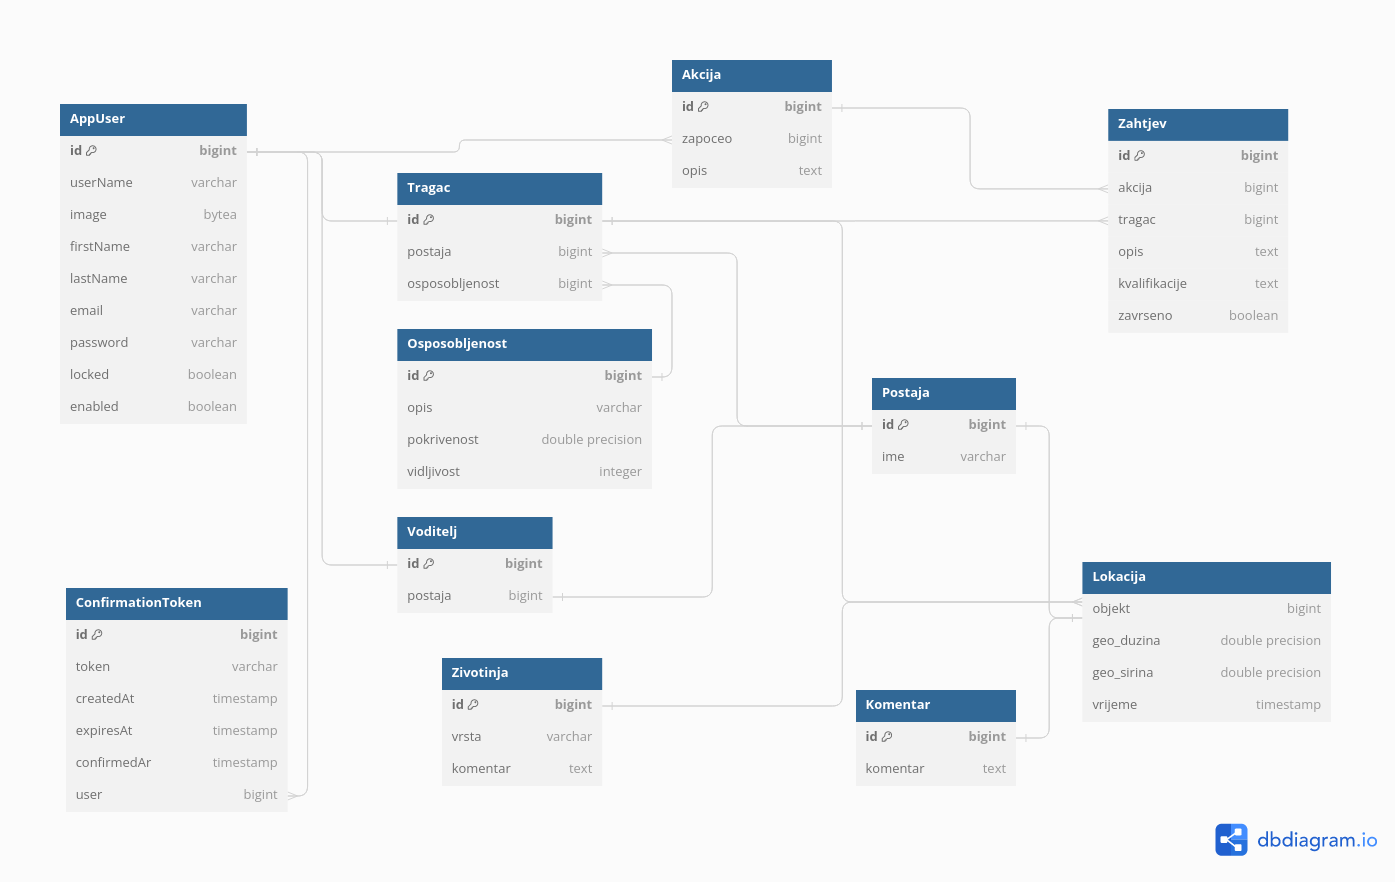
\includegraphics[scale=0.35]{dijagrami/dijagram_baze_podataka.png}
					\centering
					\caption{Dijagram baze podataka}
					\label{fig:promjene}
				\end{figure}
			\eject
			
			
		\section{Dijagram razreda}
		Dijagram razreda podijeljen je zbog bolje preglednosti na tri dijela: Controllers, Models i DTO. Prikazane su veze koje ostvaruju razredi unutar istog dijela dijagrama, a odnosi između razreda u različitim dijelovima mogu se zaključiti iz tipova atributa. Metode korištene u Controller razredima vraćaju \textit{ResponseEntity}, koji predstavlja HTTP odgovor, ili samo kod odgovora HTTP-a. U svom radu koriste objekte za prijenos podataka (DTO) i ostvaruju komunikaciju s klijentskom stranom.
			
			\begin{figure}[H]
				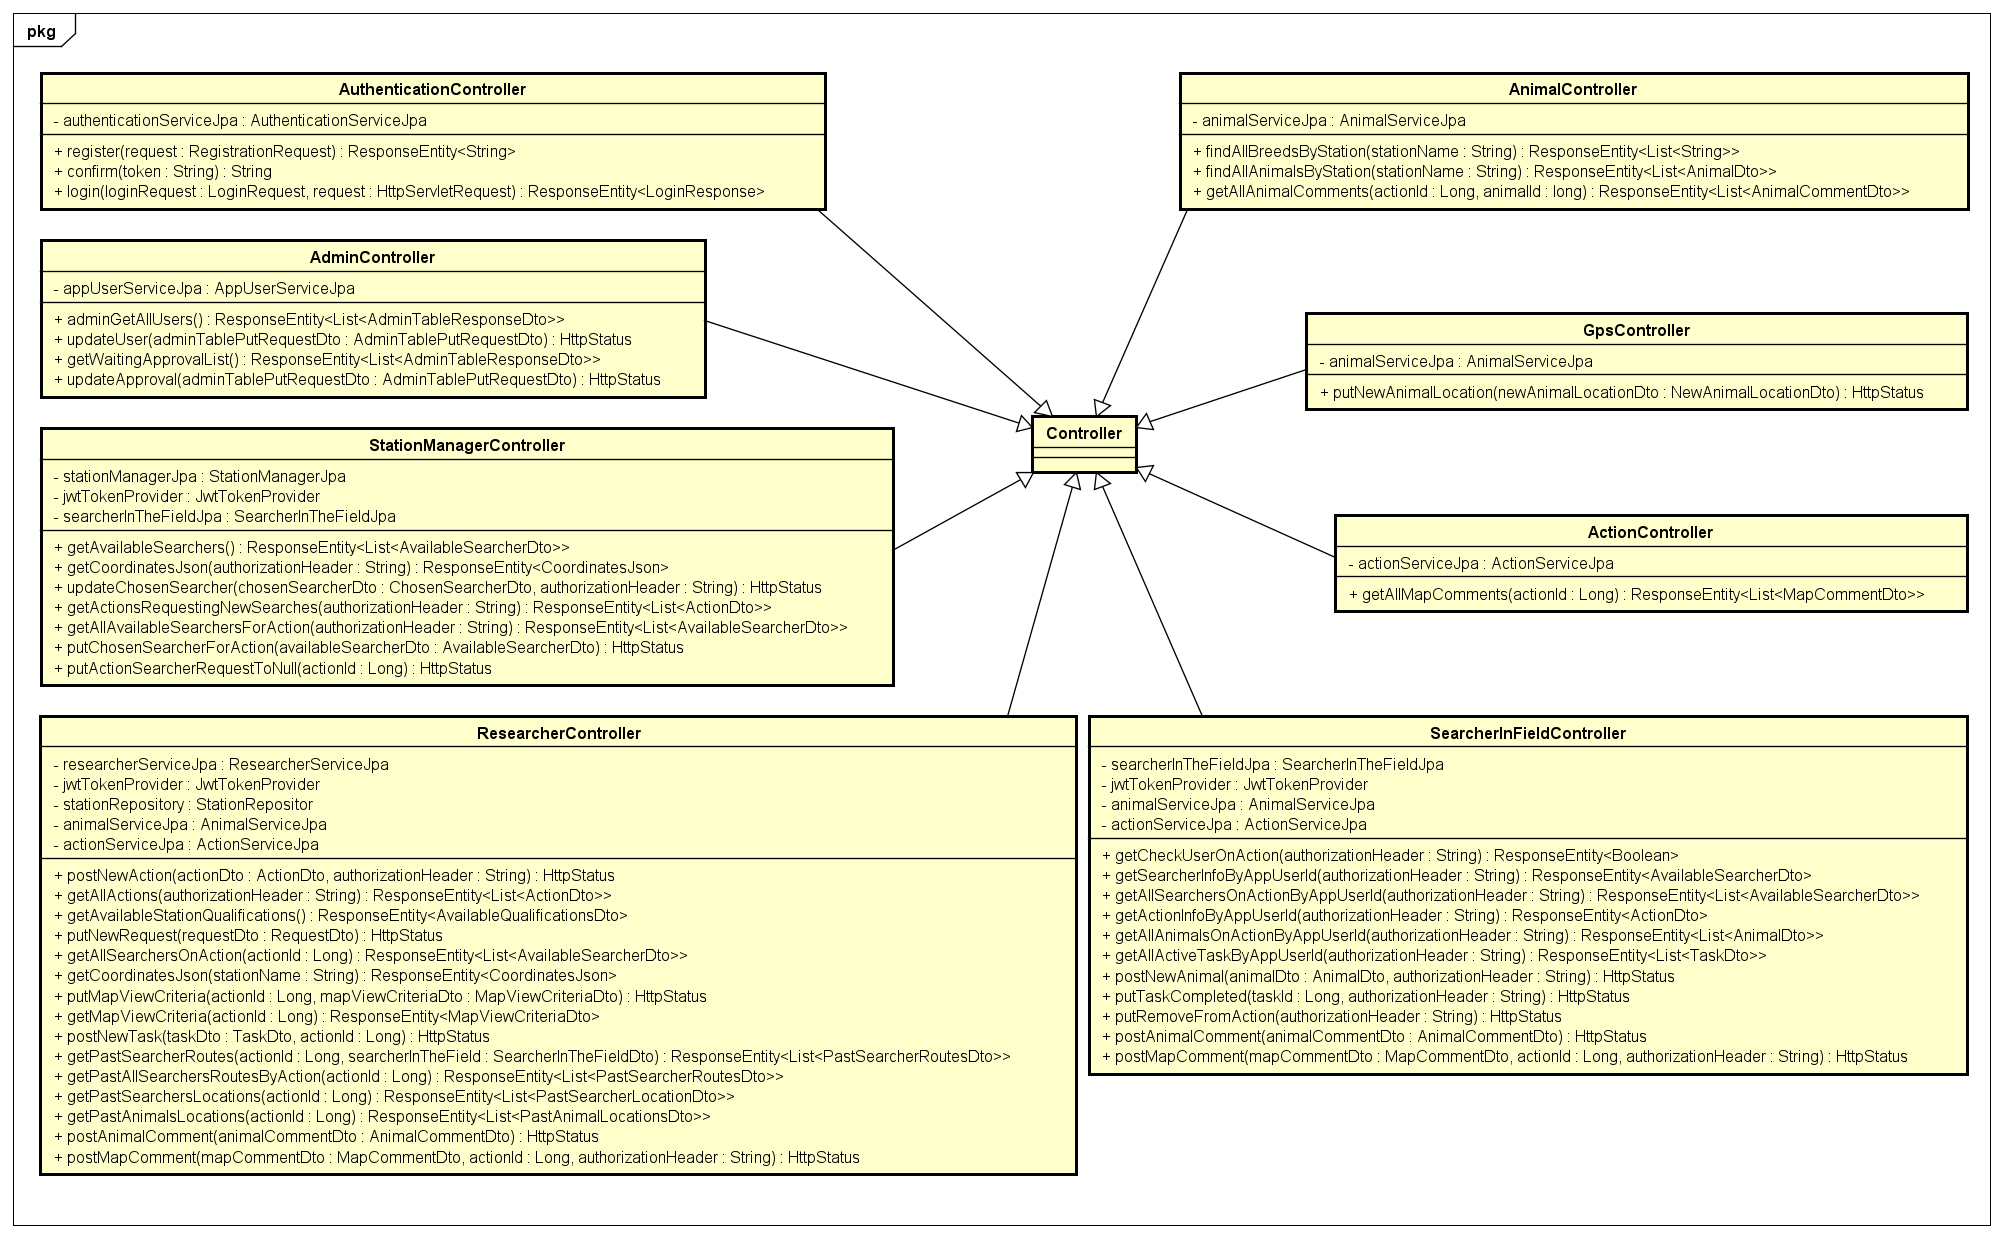
\includegraphics[scale=0.5]{dijagrami/Controllers.png} 
				\centering
				\caption{Dijagram razreda - dio Controllers}
				\label{fig:promjene}
			\end{figure}
			
			\begin{figure}[H]
				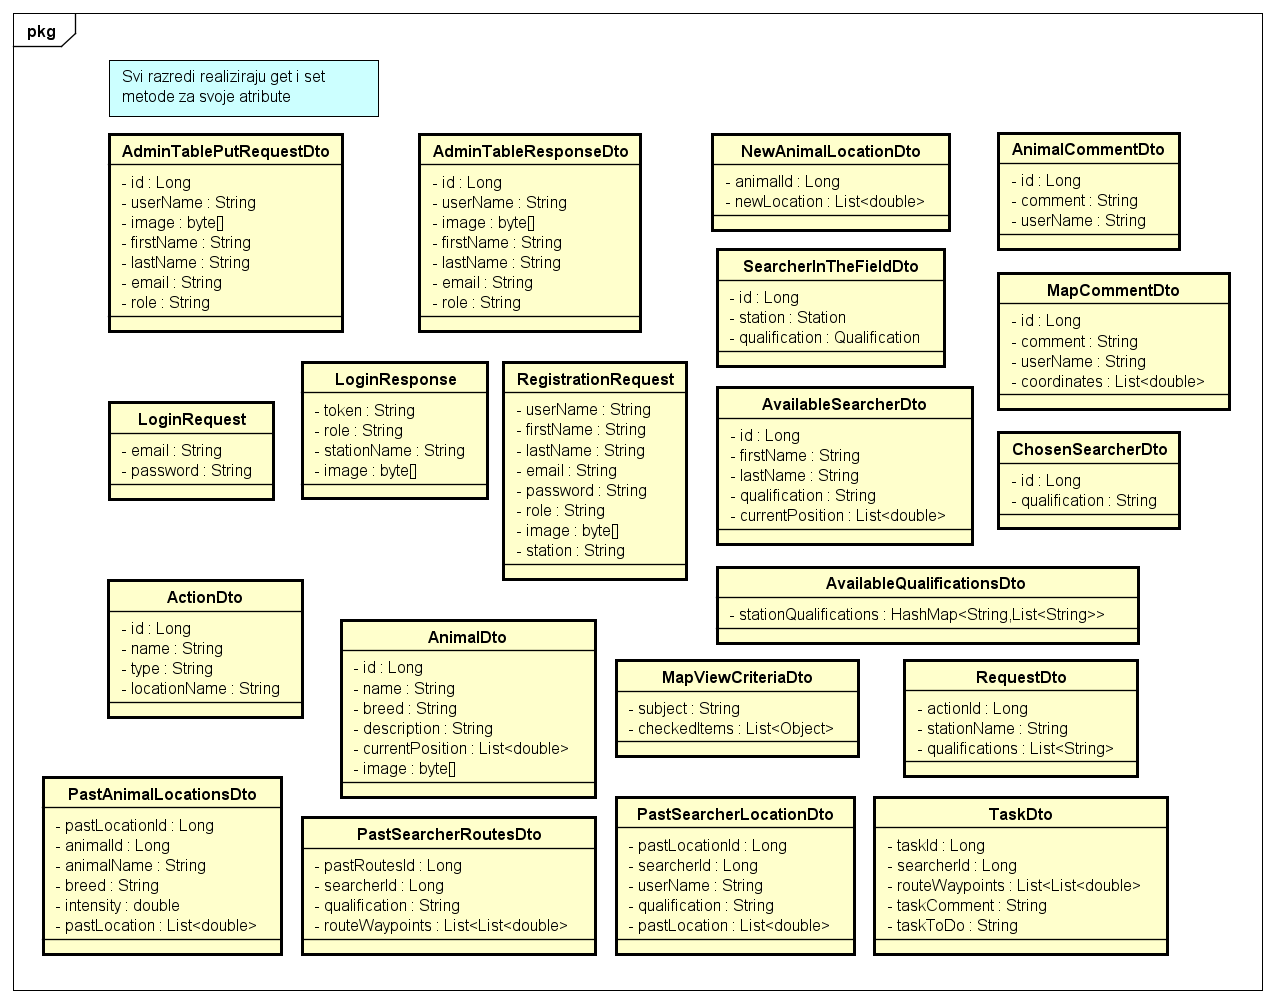
\includegraphics[scale=0.5]{dijagrami/DTO.png} 
				\centering
				\caption{Dijagram razreda - dio DTO}
				\label{fig:promjene}
			\end{figure}
			
			\begin{figure}[H]
				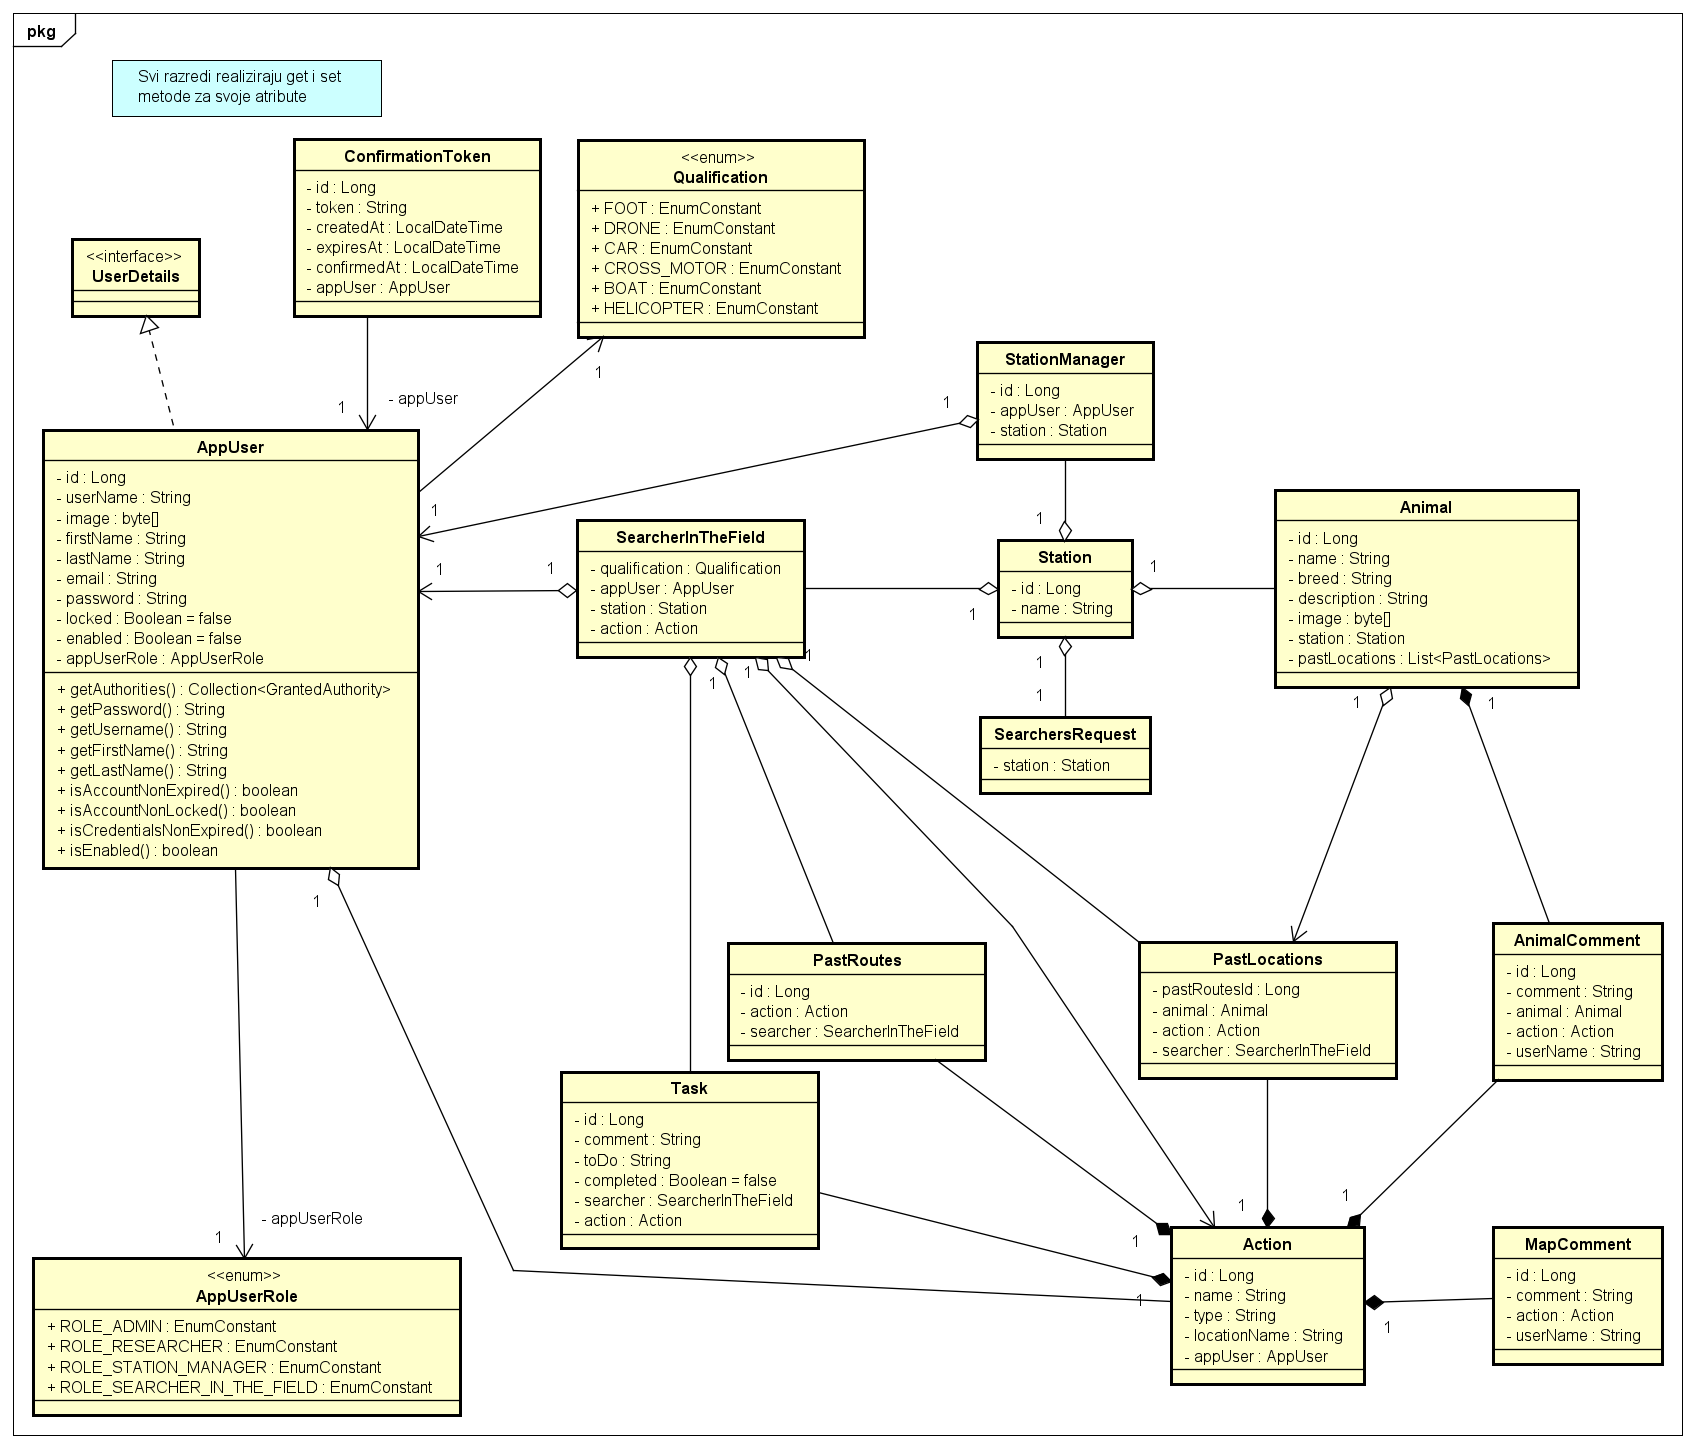
\includegraphics[scale=0.5]{dijagrami/Model.png} 
				\centering
				\caption{Dijagram razreda - dio Models}
				\label{fig:promjene}
			\end{figure}
			
			
			\eject
		
		\section{Dijagram stanja}
			
			
			\textbf{\textit{dio 2. revizije}}\\
			
			\textit{Potrebno je priložiti dijagram stanja i opisati ga. Dovoljan je jedan dijagram stanja koji prikazuje \textbf{značajan dio funkcionalnosti} sustava. Na primjer, stanja korisničkog sučelja i tijek korištenja neke ključne funkcionalnosti jesu značajan dio sustava, a registracija i prijava nisu. }
			
			
			\eject 
		
		\section{Dijagram aktivnosti}
			
			\textbf{\textit{dio 2. revizije}}\\
			
			 \textit{Potrebno je priložiti dijagram aktivnosti s pripadajućim opisom. Dijagram aktivnosti treba prikazivati značajan dio sustava.}
			
			\eject
		\section{Dijagram komponenti}
		
			\textbf{\textit{dio 2. revizije}}\\
		
			 \textit{Potrebno je priložiti dijagram komponenti s pripadajućim opisom. Dijagram komponenti treba prikazivati strukturu cijele aplikacije.}